\documentclass[11pt,a4paper]{article}
\usepackage[nohead]{geometry}
\usepackage{amsmath,amsfonts,physics}
\geometry{left=1in,right=1in,top=0.6in,bottom=1in}
\usepackage[capitalise,noabbrev]{cleveref}
\usepackage[bottom]{footmisc}
\usepackage{multicol}
\usepackage{todonotes}

\usepackage{tikz}
\usetikzlibrary{shapes, calc, decorations, automata}
\tikzstyle{midnode}=[
    draw=blue!70,   % draw the border with 70% transparent blue
    rectangle,      % the shape of the node is a rectangle
    fill=blue!10,   % fill the box with 20% blue
    text width=1cm,
    text centered]

\tikzstyle{smallnode}=[
    draw=blue!70,   % draw the border with 70% transparent blue
    rectangle,      % the shape of the node is a rectangle
    fill=blue!10,   % fill the box with 20% blue
    text width=0.4cm,
    text centered]

\crefformat{section}{\S#2#1#3}
\crefformat{subsection}{\S#2#1#3}
\crefformat{subsubsection}{\S#2#1#3}

\usepackage{listings}
\lstdefinelanguage{julia}{
  basicstyle=\small\ttfamily,
  showspaces=false,
  showstringspaces=false,
  keywordstyle={\textbf},
  morekeywords={if,else,elseif,while,for,begin,end,quote,try,catch,return,local,abstract,function,generated,macro,ccall,finally,typealias,break,continue,type,global,module,using,import,export,const,let,bitstype,do,in,baremodule,importall,immutable},
  escapeinside={~}{~},
  morecomment=[l]{\#},
  commentstyle={},
  morestring=[b]",
}
\lstset{language=julia, numbers=left, numberstyle=\tiny, mathescape=true}

\setlength{\columnseprule}{0.4pt}
\setcounter{footnote}{1}
\title{Nordsieck Form Implementation Note}
\author{Yingbo Ma\thanks{Email: \tt{mayingbo5@gmail.com},
                         GitHub: \tt{@YingboMa}}}
\date{April 2018}

\begin{document}
\maketitle
%\tableofcontents

\section*{Notations}
\begin{multicols}{2}
  \begin{itemize}
    \item For any variable $X$, let $X_n$ denote the $n$-th step of the variable $X$.
    \item For any variable $X$, let $\hat{X}$ denote the predicted value of the variable $X$.
    \item Let $\otimes$ denote the Kronecker product.
    \item Let $q$ denote the order of the method.
    \item Let $u$ denote a vector of dependent variables.
    \item Let $t$ denote a scalar independent variable.
    \columnbreak
    \item Let $F$ denote the vector equation for a ordinary differential equation
      $u' = F(u, t)$.
    \item Let $z_n$ denote the Nordsieck vector, which is
      \[
        z_n = \left[\frac{u_n}{0!}, h\frac{u_n'}{1!}, h^2\frac{u_n''}{2!},
        \cdots, h^q\frac{u_n^{(q)}}{q!}\right]^T
      \]
    \item Let $A(q)$ denote a $(q+1)\times (q+1)$ Pascal triangle matrix (lower
      triangular).
    \item Let $P(q)$ denote a $(q+1)\times (q+1)$ Pascal triangle matrix (upper
      triangular).
  \end{itemize}
\end{multicols}

\section{The General Form of Nordsieck Methods}
In the Nordsieck formulation of multi-step methods we first need to find
interpolating polynomial $\pi_{n-1}$ and $\pi_n$, which is going to be
introduced in \cref{sec:adams} for Adams-Bashforth method and
\cref{sec:bdf} for BDF(Backward differentiation formula) method. The
predictor part in the Nordsieck formulation is independent from the choice of
interpolating polynomials. This this subsection, we going to solely discuss the
predictor.

A Nordsieck vector is a vector that is in the form of
\begin{equation}
  z_n = \left[\frac{u_n}{0!}, h\frac{u_n'}{1!}, h^2\frac{u_n''}{2!},
  \cdots, h^q\frac{u_n^{(q)}}{q!}\right]^T
\end{equation}
Note that this derivatives $y_{n-1}^{(j)}$ are not the exact values of
$F^{(j)}_{n-1}$, and they are the approximations from a interpolation
polynomial $\pi_{n-1}^{(j)}(t_{n-1})$ with the order of accuracy
$\mathcal{O}(h^{q+1})$ if $y_{n-1}$ has the correct order. Now, we can
propagate the $z_{n-1}$ to $\hat{z}_{n}$ by a Pascal triangle matrix, which in
essence, a Taylor expansion. Thus, the formula for the predictor reads
\begin{equation}
  \hat{z}_n = z_{n-1}P(q).
\end{equation}
While one can construct the Pascal matrix explicitly
\begin{lstlisting}
P(q) = [i>=j ? binomial(i,j) : 0 for i in 1:q+1, j in 1:q+1]
\end{lstlisting}
and perform matrix-matrix multiply to get $z_n$, a much efficient method is to
write a \texttt{for} loop.
\begin{lstlisting}
for i in 1:q, j in q:-1:i
  z[j] = z[j] + z[j+1]
end
\end{lstlisting}

Now we have a formulation for the predictor that is based on Taylor expansion.
For the corrector, we are going to make use of an interpolating polynomial
$\pi_{n}$ with order $q$ or less.

%However, another perspective of those multi-step numerical schemes are from
%polynomials with constraints directly. That is, a polynomial with $L\equiv q+1$
%constraints one can full encode ~\cref{eq:Adams_int} and~\cref{eq:BDF_int}.

\section{BDF Methods} \label{sec:bdf}
The backward differentiation formula methods are usually
presented as
\begin{equation} \label{eq:BDF_int}
  \sum_{j=1}^q j^{-1}\nabla^ju_{n+1} = hF_{n+1},
\end{equation}
where $\nabla$ is a backward difference operator\footnote{A backward
difference operator has the recurrence relation of
\[
  \nabla^0u_n = u_n,\quad \nabla^{j+1}u_n = \nabla^ju_n-\nabla^ju_{n-1}.
\]}.
Similar to the Adams family, BDF methods can be thought as a polynomial
interpolation that fulfills $L\equiv q+1$ conditions
\begin{align}
  \pi_{n-1}(t_{n-i})&=u_{n-i}\qq{where} i=1,2,\cdots,q \\
  \pi_{n-1}'(t_{n-1})&=F_{n-1},
\end{align}
also, we can construct a corrector polynomial by $L+1$ conditions
\begin{align}
  \pi_{n}(t_{n-i})&=u_{n}\qq{where} i=0,1,\cdots,q \\
  \pi'_{n}(t_{n})&=F_{n}.
\end{align}
Define $\hat{u}_n = \pi_{n-1}(t_n)$ and $\hat{u}'_n = \pi'_{n-1}(t_n)$. Note
that $r=\hat{u}'_n - F_n$ does not usually vanish, so one can use it as a
residual to calculate corrected $u_n$. We define the corrected Nordsieck vector
by
\begin{equation}
  z_n = \left[\frac{u_n}{0!}, h\frac{u_n'}{1!}, h^2\frac{u_n''}{2!},
  \cdots, h^q\frac{u_n^{(q)}}{q!}\right]^T,\quad u_n^{(j)}\equiv
  \pi_n^{(j)}(t_n).
\end{equation}

Now, we shall compute the relation between $\hat{z}_n$ and $z_n$. Define a
polynomial
\begin{equation}
  \Delta_n(t) = \pi_n(t) - \pi_{n-1}(t),
\end{equation}
and a correction quantity
\begin{equation}
  e_n = u_n - \hat{u}_n = \pi_n(t) - \pi_{n-1}(t).
\end{equation}
We have the relation
\begin{equation}
  \Delta_n(t_{n-i}) = 0, \quad i=1,2,\cdots,q,
\end{equation}
which leads to
\begin{equation}
  \Delta_n(t) = \Pi_{i=1}^q \frac{t-t_{n-i}}{t_n-t_{n-i}}e_n.
\end{equation}
We have
\begin{align}
  \Lambda_n(x) &= \Pi_{i=1}^q (1+\frac{x}{\Xi_i}) = \sum_{j=0}^{q}l_jx^{j}, \quad x=\frac{t-t_n}{h},\;
  \Xi_i = \frac{t_n-t_{n-i}}{h} \\
  \Delta_n(t) &= \Delta_n(t_n+hx) = \Delta_n(x)e_n.
\end{align}
Then, we have
\begin{align}
  h^j\pi_n^{(j)}(t_n)/j! - h^j\pi_{n-1}^{(j)}(t_n)/j! = h^j\Delta_n^{(j)}/j! =
  \Lambda_n^{(j)}(0)e_n/j! = l_je_n.
\end{align}
Define
\begin{equation}
  l = [l_0, l_1, \cdots, l_q],
\end{equation}
then
\begin{equation}
  z_n = \hat{z}_n + e_n l.
\end{equation}
This simple relation is used to calculate the corrected value.

For the BDF method, the vector $l$ can be calculated as
\begin{equation}
  l_1 = 1,\; l_1 = \sum_{i=1}^q \Xi_i^{-1},\; l_q =
  (\Xi_1\Xi_2\cdots\Xi_1)^{-1}.
\end{equation}
We also have a two-term recurrence
\begin{equation}
  l_j(q) = l_j(q-1) + \frac{l_{j-1}(q-1)}{\Xi_q}.
\end{equation}

\section{Adams Methods} \label{sec:adams}
The Adams methods are usually presented as
\begin{equation} \label{eq:Adams_int}
  u_{n+1} = u_n + \int_{t_n}^{t_{n+1}} P(\tau) \dd{\tau},
\end{equation}
where $P(t)$ is an interpolation polynomial through points $t_i, F_i$ for
$i=n-q+1,\cdots,n$.
Explicit Adams methods can be thought as a polynomial interpolation that
fulfills $L\equiv q+1$ conditions
\begin{align} \label{eq:adams1}
  \pi_{n-1}'(t_{n-i})&=F_{n-i}\qq{where} i=1,2,\cdots,q \\
  \pi_{n-1}(t_{n-1})&=u_{n-1},
\end{align}
while the implicit Adams methods are the same with polynomials that fulfills
$L+1$ conditions
\begin{align} \label{eq:adams2}
  \pi_{n}(t_{n-i})'&=F_{n-i}\qq{where} i=0,1,\cdots,q-1 \\
  \pi_{n}(t_{n-1})&=u_{n-1} \\
  \pi_{n}(t_{n})&=u_{n}.
\end{align}
Here, we define that $u'_n$ is $F_n$. Note that those conditions are equivalent
with the classical linear multi-step form
\begin{equation}
  u_n = u_{n-1} h_n\sum_{i=0}^{q-1}\beta_{ni}u'_{n-i}.
\end{equation}
Here the coefficients $\beta_{ni}$ dependents on $h_j$ and order $q$. Now,
define $\hat{u}_n = \pi_{n-1}(t_n)$ and $\hat{u}'_n = \pi'_{n-1}(t_n)$. We have
\begin{equation} \label{eq:nl_adams}
  hu'_n = hF_n = h\hat{u}'_n + \Delta_n l_1,
\end{equation}
where $\Delta_n = \pi_n - \pi_{n-1}, h=h_n$ and $l_1 =
\beta_{n0}^{-1}$. The $\Delta$ vector in \cref{eq:nl_adams} can be solved by
function iteration.
\begin{lstlisting}
# Zero out the difference vector
Delta .= zero(eltype(Delta))
# `k' is a counter for convergence test
k = 0
# Start the functional iteration & store the difference into `Delta'
while true
  @. ratetmp = inv(l[2])*muladd(dt, ratetmp, -z[2])
  @. integrator.u = ratetmp + z[1]
  @. Delta = ratetmp - Delta
  del = norm(cache.Delta)
  # Convergence test
  test_rate <= one(test_rate) && return true
  # Divergence criteria
  (k == max_iter) || (k >= 2 && del > div_rate * del_prev) && return false
  del_prev = del
  integrator.f(ratetmp, integrator.u, p, dt+t)
end
\end{lstlisting}

From \cref{eq:adams1} and \cref{eq:adams2}, we see that
\begin{equation}
  \Delta_n(t_n) = u_n - \hat{u}_n \equiv e_n,\; \Delta_n(t_{n-1}) = 0,\;
  \Delta'_n(t_{n-1}) = 0, \qq{where} i=1,2,\cdots,q-1.
\end{equation}
Thus we have
\begin{equation}
  \Delta_n(t) = \Delta_n(t_n+hx) = \Lambda_n(x)e_n, \quad x = (t-t_n)/h,
\end{equation}
where $\Lambda_n$ is a scalar polynomial that fulfills the conditions
\begin{equation}
  \Lambda_n(0)=1,\; \Lambda_n(-1) = 0,\; \Lambda'_n(\Xi_i) = 0,\qq{where}
  i=1,2,\cdots,q-1,\; \Xi_i \equiv (t_n-t_{n-i})/h.
\end{equation}
Hence, we can write $\Lambda_n$ as
\begin{equation}
  \Lambda_n(x) = \frac{\int_{-1}^x\prod_{i=1}^{q-1} (u+\Xi_i) \dd{u}}
          {\underbrace{\int_{-1}^0\prod_{i=1}^{q-1} (u+\Xi_i)
          \dd{u}}_\text{constant normalization}}
               = \sum_{j=0}^{q} l_jx^j.
\end{equation}
We can compute the vector $l_j$ by first calculating the coefficients of
$\prod_{i=1}^{q-1} (u+\Xi_i)$ and integrate it with some normalization. Here is
an implementation which uses Vieta's formulas,
\begin{equation}
  \sum_{1\leq i_{1}<i_{2}<\cdots <i_{k}\leq n}x_{i_{1}}x_{i_{2}}\cdots
  x_{i_{k}}=(-1)^{k}l_{n-k},
\end{equation}
where $x_j$ is the $j$-th roots of a polynomial. Here is the Julia
implementation for computing $\int_{-1}^x\prod_{i=1}^{q-1} (u+\Xi_i) \dd{u} =
\sum_{i=1}^{q-1} m_ix^i$.
\begin{lstlisting}
  # compute coefficients from the Newton polynomial
  m[1] = ONE
  for j in 1:order-1
    Xi_inv = dt / dtsum
    for i in j:-1:1
      m[i+1] += m[i] * Xi_inv
    end
    dtsum += tau[j+1]
  end
\end{lstlisting}
Next, we need to have a routine to integrate the coefficients of this
polynomial. The implementation reads
\begin{lstlisting}
# This function computes the integral, from -1 to 0, of a polynomial
# `P(x)` from the coefficients of `P` with an offset `k`.
function int01dx(a, deg, k)
  int = zero(eltype(a))
  sign = one(eltype(a))
  for i in 1:deg
    int += sign * a[i]/(i+k)
    sign = -sign
  end
  return int
end
\end{lstlisting}
Finally, we can combine them, we then have
\begin{lstlisting}
function calc_coeff!(cache::T) where T
  @unpack m, l, tau = cache
  ZERO, ONE = zero(m[1]), one(m[1])
  dtsum = dt = tau[1]
  order = cache.step
  # normalization
  M0 = int01dx(m, order, 0)
  M0_inv = inv(M0)
  l[1] = ONE
  for i in 1:order
    l[i+1] = M0_inv * m[i] / i
  end
end
\end{lstlisting}
\todo[inline]{Order increase/decrease and error estimation. Maybe stiffness
detection.}

\section{Code organization}
\todo[inline]{This still is a placeholder.}
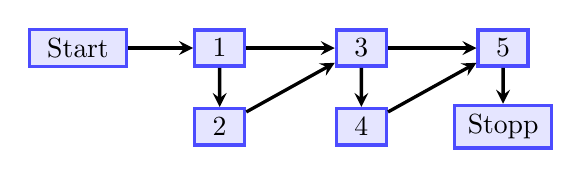
\begin{tikzpicture}[->,>=stealth,auto, very thick, scale=5]
        % Draw the vertices.
        \node[midnode] (s) {Start};
        \node[smallnode, right of=s, node distance=1.8cm] (a) {1};
        \node[smallnode, below of=a] (b) {2};
        \node[smallnode, right of=a, node distance=1.8cm] (c) {3};
        \node[smallnode, below of=c] (d) {4};
        \node[smallnode, right of=c, node distance=1.8cm] (e) {5};
        \node[midnode, below of=e] (x) {Stopp};

        % Connect vertices with edges
        \path (s) edge node {} (a);
        \path (a) edge node {} (c);
        \path (a) edge node {} (b);
        \path (b) edge node {} (c);
        \path (c) edge node {} (d);
        \path (c) edge node {} (e);
        \path (d) edge node {} (e);
        \path (e) edge node {} (x);
\end{tikzpicture}

\end{document}
